% {{{
\documentclass[12pt]{article}
\usepackage[tmargin=0.75in,bmargin=0.75in,lmargin=0.9in,rmargin=0.9in]{geometry}

\usepackage{amsmath}
\include{latexsym}
\include{amssymb}
\usepackage{enumitem}
\usepackage[symbol, hang]{footmisc}
\usepackage{indentfirst}
\usepackage{amssymb}
\usepackage{graphicx,psfrag}

\def\F{\mathcal{F}}
\def\M{\mathcal{M}}
\def\dimspec{\mathfrak{D}}
\def\htop{h_{top}}
\def\trans{\mathcal{T}}
\def\G{\mathcal{G}}
\newcommand{\Z}{\mathbb{Z}}
\pagenumbering{gobble}
\def\O{\mathcal{O}}

\newcommand\NoIndent[1]{%
  \begingroup
  \par
  \parshape0
  #1\par
  \endgroup
}
% }}}

% Title {{{
\begin{document}

\begin{center}
{\large \bf CompMethods }   \\ \large pset7 \\ Ephraim Sutherland
\end{center}
% }}}

\subsection*{Problems}

\begin{enumerate}

	\item we know the actual answer (computed analytically) is: $E(\mu, \sigma) = 4.4816890703380645$
		\\When we run gaussian-hermite with  $n=2$, we have $gaussianHermite(g, 2) = 4.194528049465325$
		\\When we run gaussian-hermite with  $n=10$, we have $gaussianHermite(g, 10) = 4.481689070332898$
		Thus we can see although gaussianHermite is surprisingly quite close with 2 points, when we switch to $n=10,$ our answer is almost exactly the same as the analytic solution.

	\item
		\begin{enumerate}
			\item $v_0(b) = 0.46804469425529605$	
				\\ $g_0(b) = 1.4232759265450888e^{-8}$
				\begin{center}
					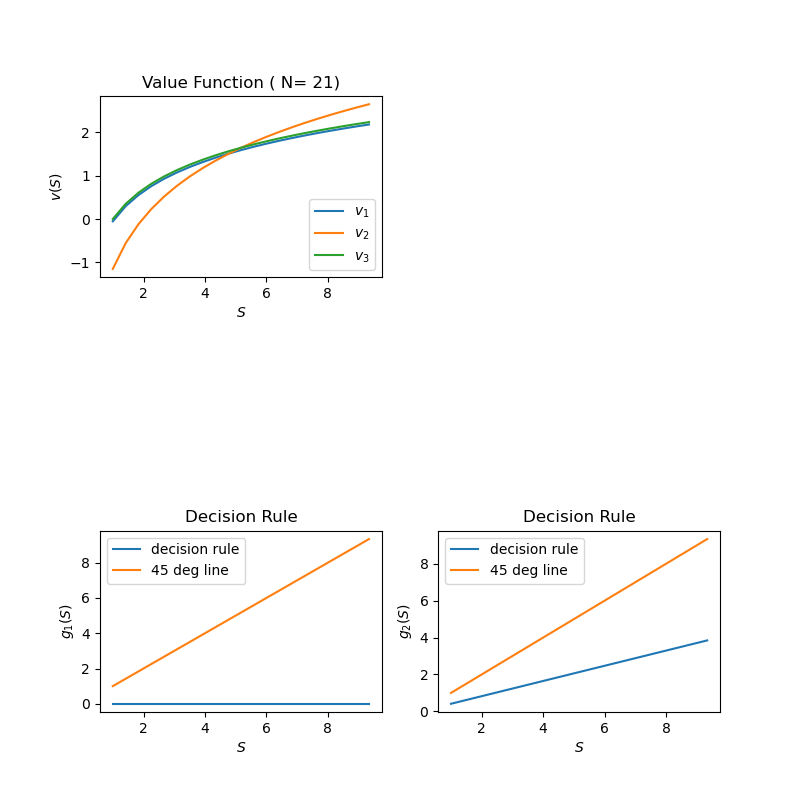
\includegraphics[width=\textwidth]{2_a.png}
				\end{center}
			\item Running the simulation 10 times.	
				\begin{center}
					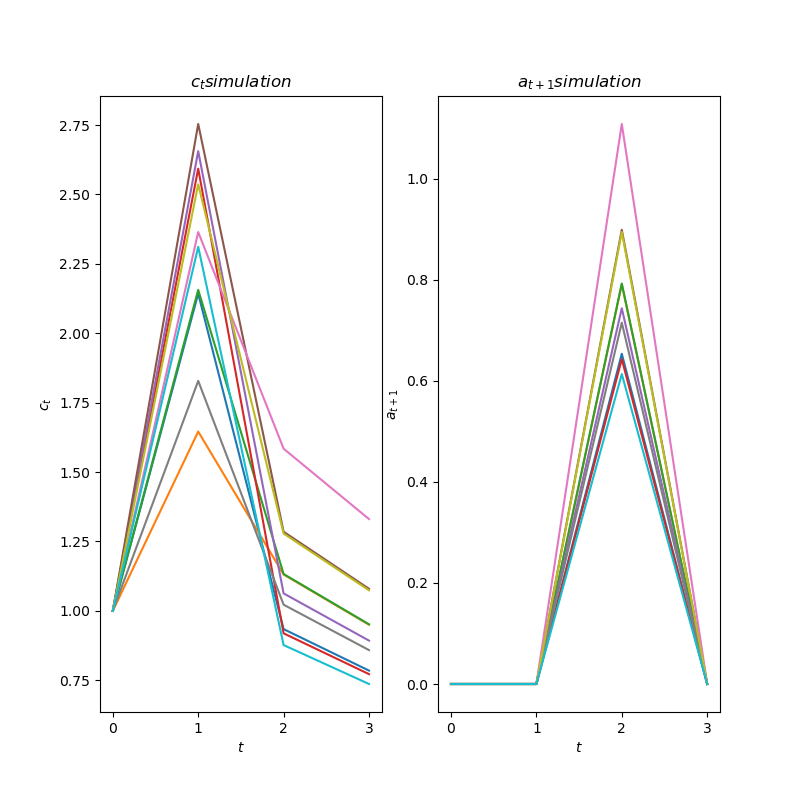
\includegraphics[width=\textwidth]{2_b.png}
				\end{center}

		\end{enumerate}
\end{enumerate} 

\end{document}


